\documentclass{tufte-handout}
\title{Applied Algorithms\newline Mandatory Assignment \#$2$}

\usepackage[utf8]{inputenc}

\usepackage{graphicx} % for handling images

\usepackage{amsmath}
\usepackage{booktabs}
\usepackage{microtype}

\usepackage{pgfplots} % layout and margin handling
\pgfplotsset{width=10cm,compat=1.13}

\usepackage{booktabs}
\usepackage{tcolorbox}

% Graphics
\usepackage{graphicx}
\usepackage{subfig}

% Code formatting   
\usepackage{listings}
\lstset{
   language=java,
   extendedchars=true,
   basicstyle=\footnotesize\ttfamily,
   showstringspaces=false,
   showspaces=false,
   numbers=left,
   numberstyle=\footnotesize,
   numbersep=9pt,
   tabsize=2,
   breaklines=true,
   showtabs=false,
   frame=single,
   extendedchars=false,
   inputencoding=utf8,
   captionpos=b
}

\begin{document}

\thispagestyle{empty}

\maketitle

\includegraphics[width=\textwidth]{figs/logo_en.png}

\vspace{10mm}\noindent %10mm vertical space

\begin{center}
{\LARGE Distinct elements using hashing}
\end{center}

\vspace{5mm}\noindent %10mm vertical space

\begin{table}[!h]
\centering
\begin{tabular}{cc}
\multicolumn{2}{c}{Authors}                                   \\ \hline
\multicolumn{1}{c|}{\textbf{Hugo Brito}} & \textbf{René Haas} \\
\multicolumn{1}{c|}{\href{mailto:hubr@itu.dk}{hubr@itu.dk}}         & \href{mailto:renha@itu.dk}{renha@itu.dk}       \\ \hline
\end{tabular}
\end{table}

\vspace{5mm} %10mm vertical space

%\newpage

\section{Introduction}

In this report we show our findings with the HyperLogLog algorithm for estimating distinct elements.
All our experiments are reproducible and can be rerun by using the {\tt Makefile}. If the reader wishes to rerun our experiments simply {\tt cd} to the {\tt src} folder and type {\tt make}.

\section{\textbf{Exercise 1.}}
In this first exercise we are given a matrix $A\in\{0,1\}^{b\times k}$ where $b=k=32$. We are asked to implement the hash function
\begin{align*}
  h(x)_i = \sum_{j=1}^b A_{i,j}x_j \mod 2
\end{align*}
We implement the function in Java (see {\tt Ex1.java})
with the following code:

\begin{lstlisting}
public static int h(int x) {
    int res = 0;
    for (int i = 0; i < A.length; i++) {
        res += (Integer.bitCount(A[i] & x) % 2) << (31-i);
    }
    return res;
}
\end{lstlisting}
\noindent We start by calculating the bit-wise {\tt \&} (and) operation between $x$ and the rows of $A$. The result of this operation is a binary number which is equivalent to a vector consisting of the element-wise products of the components of $x$ and the $i^{th}$ row of $A$. We then count the sum with {\tt Integer.bitCount} and then take the modulus $2$ of that number. This gives us an integer which is either $0$ or $1$. We make this the integer the $j$ bit in the result by using the shift operator {\tt <<}. This implementation passes the tests on CodeJudge.

\section{\textbf{Exercise 2.}}

We are asked to implement the function $\rho(y) = \min\{i\ |\ y_{k-i}=1\}$. We do this the easy way in Java by simply using the {\tt Integer.numberOfLeadingZeros} function from the Java standard library and adding $1$ to the result. We add $1$ because we are interested in the first position that is not $0$. The implementation can be found on the {\tt Ex2.java} file and looks like the following:

\begin{lstlisting}
public static int rho(int x) {
    if (x == 0) { throw new InputMismatchException("Zero is undefined"); }
    return Integer.numberOfLeadingZeros(x);
}
\end{lstlisting}
\noindent
It is claimed that the distribution of hash values of $\rho$ satisfies $Pr(\rho(y)=i) = 2^{-i}$.
In Figure \ref{fig:ex2} we show a histogram over the values of $\rho(x)$ for $x \in \{1,\cdots,10^6\}$. We find that there is direct experimental support for this claim, although in reality $Pr(\rho(y)=i)=2^{-i}/2$. This is verified experimentally in Fig \ref{fig:ex2} and the factor of $1/2$ is also theoretically necessary since $\sum_{i=1}^{\infty} = 2$ and a probability distributions must be normalised.

\begin{figure}[h!]
  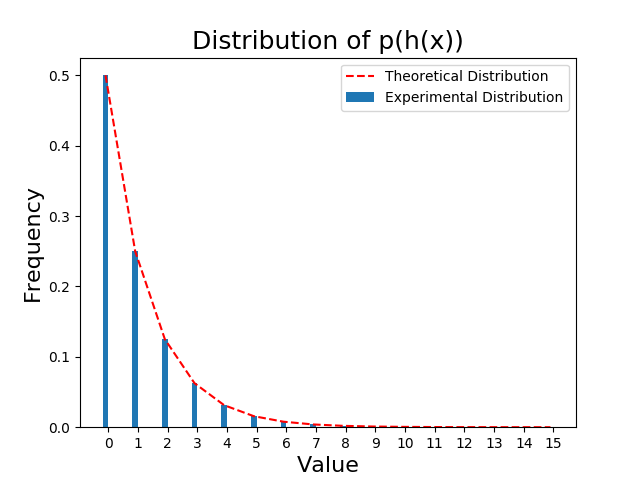
\includegraphics[width = \textwidth]{figs/ex2-hist}
  \caption{Histogram of $\rho(x)$ for $x \in \{1,\cdots,10^6\}$}
  \label{fig:ex2}
\end{figure}

\section{\textbf{Exercise 3.}}
% Exercise 3. Implement this algorithm with m = 1024 and k = 32. Test it on the input sequence 106; : : : ; 2  106 �� 1 with 1 million distinct items: How many distinct elements are reported by your implementation? (Add this number to your report.)

We have implemented the algorithm and this implementation for the values $m = 1\ 024$ and $k = 32$ can be found in {\tt Ex3.java} file. This file also passes all instances of CodeJudge.
\\\noindent
For the given $m$, $k$ and the given sequence of distinct integers $x \in \{10^6,\cdots,2\times 10^6 - 1\}$ the implementation of this algorithm estimates that there are $973\ 089,272$ distinct values. The error\footnote{Taken from \href{https://www.thoughtco.com/how-to-calculate-percent-error-609584}{thoughtco.com}} is then $|1\ 000\ 000 - 973\ 089,272| = 26\ 910,728$, which translates to $2,69\%$.

\section{\textbf{Exercise 4.}}

% As alluded to earlier, the space usage of the HyperLogLog counter influences its estimation error. In the last exercise, we want to experimentally find out how strong this influence is.

% Write an input generator that takes as input an integer n and a seed seed on standard input and outputs a list of n random 32-bit integers from a random integer generator using seed seed. Describe and run an experiment that gives a graphical representation of the connection of m and the estimation error. A recommended representation is a histogram plot over the distinct element count reported by the algorithm. Try at least 3 dierent values of m.

% we have the table and want to correlate the number of times for each m that an estimation falls inside the first sigma, the second sigma, or none. we have the columns that report true or false for that.

% we can make a graph out of that table

\noindent Lastly, we wanted to find the co-relation between the space usage of the HyperLogLog counter influences its estimation error.\\
\bigskip \noindent
The file {\tt Ex4.java} implements the input generator to be used by the HyperLogLog algorithm. We wanted to be certain that the algorithm would always estimate the number of distinct integers and compare that estimation to the real number of distinct integers. In order to achieve this machinery, the above-mentioned generator would add the generated integers to set. Below the code snippet that implements this description:

\begin{lstlisting}
do {
	int i = a + random.nextInt(-a + b + 1);
	if (i != 0) { // zero cannot be used because it has no leading zeros and cannot be hashed
		integers.add(i);
    // omitted for brevity
	}			
} while (integers.size() < n);
\end{lstlisting}
\noindent
Variable description:
\begin{itemize}
    \item {\tt a}: The lower bound of the random generator
    \item {\tt b}: The upper bound of the random generator
    \item {\tt integers}: The set of distinct integers
    \item {\tt n}: The real number of distinct integers
\end{itemize}
\noindent
The file {\tt Experiment.java} implements experiment we designed to assess the relation between the $m$ and the estimation. It takes a set of distinct integers and $m$ as constructor parameters and outputs all the information needed to report on this relation, namely:
\begin{itemize}
    \item The estimation
    \item A {\tt boolean} value that would evaluate to {\tt true} should the estimation fall within one $\sigma$ range  
    \item A {\tt boolean} value that would evaluate to {\tt true} should the estimation fall within $2\sigma$ range 
    \item $\sigma$
    \item The lower and upper bounds of the $\sigma$ range
    \item The lower and upper bounds of $2\sigma$ range
\end{itemize}
\noindent
Finally, the file {\tt main.java} combines all the above and outputs the results to a file. In itself, it contains a {\tt long} generator that was initialised with the {\tt seed} $42$. The output of this {\tt long} generator is then used as {\tt seed} in the {\tt Ex4.java} file to generate sets of distinct integers. Once the set is created, $3$ {\tt Experiment} are instantiated with different values of $m\in\{16, 256, 1024\}$. In each iteration a new set is generated with an unused {\tt seed} (we garantee this by keeping a set {\tt usedSeeds}) this is passed to the $3$ instances. In order to achieve significant data, this process is repeated $100\ 000$ times.

\begin{figure}[!h]
  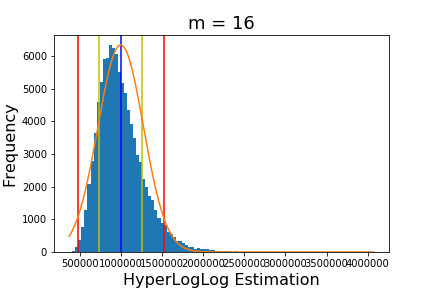
\includegraphics[width = \textwidth]{figs/ex416}
  \caption{HiperLogLog estimation distribution for $m = 16$ over $100\ 000$ distinct sets of $1\ 000\ 000$ distinct integers}
  \label{fig:16}
\end{figure}
\noindent In figures \ref{fig:16}, \ref{fig:256} and \ref{fig:1024} we see histograms that resulted from these experiments. In the figures the yellow vertical lines represent $n(1\pm\sigma)$ range and the red lines represent $n(1\pm2\sigma)$ range. We have also fitted a Gaussian distribution and plotted that on top of the histogram in orange.
\begin{figure}[h!]
  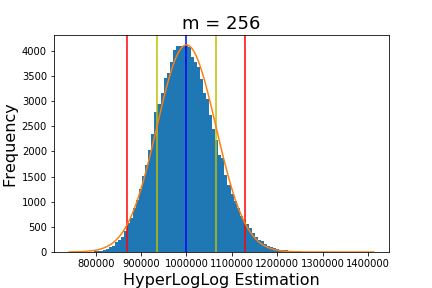
\includegraphics[width = \textwidth]{figs/ex4256}
  \caption{HiperLogLog estimation distribution for $m = 256$ over $100\ 000$ distinct sets of $1\ 000\ 000$ distinct integers}
  \label{fig:256}
\end{figure}
\begin{figure}[h!]
  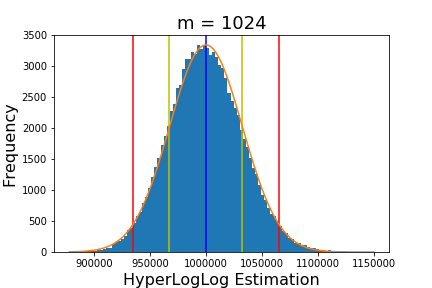
\includegraphics[width = \textwidth]{figs/ex41024}
  \caption{HiperLogLog estimation distribution for $m = 1\ 024$ over $100\ 000$ distinct sets of $1\ 000\ 000$ distinct integers}
  \label{fig:1024}
\end{figure}
% \clearpage

\noindent We can see that the error distribution follows a normal Gaussian distribution. In Table \ref{fractions} we see the fraction of runs that fall inside $n(1\pm\sigma)$ and $n(1\pm2\sigma)$ for the three different values of $m$ respectively.

\begin{table}
  \centering
  \begin{tabular}{ l | c | c | c}
                     & $m = 16$ & $m = 256$ & $m = 1024$\\ \hline
  $n(1\pm\sigma)$    & $69,453\%$ & $68,596\%$ & $68,521\%$ \\ \hline
  $n(1\pm 2\sigma)$   & $95,042\%$ & $95,476\%$ & $95,523\%$ \\ \hline
  \end{tabular}
  \caption{Fractions of runs that fall inside $n(1\pm\sigma)$ and $n(1\pm2\sigma)$ for different $m$s}
  \label{fractions}
\end{table}

\section{\textbf{Conclusion}}

The HyperLogLog algorithm is an effective strategy to estimate the cardinality of a set of integers as it does not require to keep track of the integers, saving memory space.
\noindent We could also see that  allocating to space (buckets) by increasing the size of $m$ does not influence the distribution of the error, which always follows the Gaussian distribution. It is important to mention that being $\sigma$ a function of $m$, decreasing $m$ will also increase the error range, resulting in estimations that are further away from the real value in absolute terms. Se there is some gain in for instance increasing $m$ from $16$ to $256$, but this gain is less expressive from $256$ to $1024$.

\end{document}